\section{Introduction \& contexte}

\begin{frame}{Contexte}
  \begin{block}{Wireless Sensor Network \& Low-Power and Lossy Network}
    \begin{itemize}
      \item Réseau utilisant une radio pour communiquer
      \item Systèmes embarqués
      \item Capteurs, actionneurs
    \end{itemize}
  \end{block}

  \begin{block}{Raisons technologiques}
    \begin{itemize}
      \item Réduction des couts de fabrication
      \item Réduction des besoins énergétiques
    \end{itemize}
  \end{block}

  \begin{block}{Raisons d'usages}
    \begin{itemize}
      \item Ajout de fonctionnalités de services a des objets courants
      \item Analyse des données pour fournir de l'aide à la décision
      \item Intégration centralisée
    \end{itemize}
  \end{block}

  \pnote{
    - Système embarqué existent depuis longtemps c'est quoi la différence ?
    => Approche systématique pour chaque objet car les couts sont faibles.
    => Avec des batteries standards le système peut tenir suffisamment longtemps
    }
  \pnote{
    - L'interconnexion avec des systèmes existant est aussi clé.
  }
  \pnote{
    - Les objets sont des sources d'informations et d'actions en temps réel.
  }

\end{frame}

\begin{frame}\frametitle{Motes}

  \begin{figure}[tb]
    \centering
    \includegraphics[width=\textwidth]{figures/motes.jpg}
  \end{figure}

  \pnote{
    - Mote sur support USB avec une source d'énergie pour en faire un système embarqué. 
  }
  \pnote{
    - Interconnexion en réseau
  }
  \pnote{
    - Applications simples de relevés ou d'actionneurs
  }

\end{frame}


\begin{frame}\frametitle{Testbed}

  \begin{figure}[tb]
    \centering
    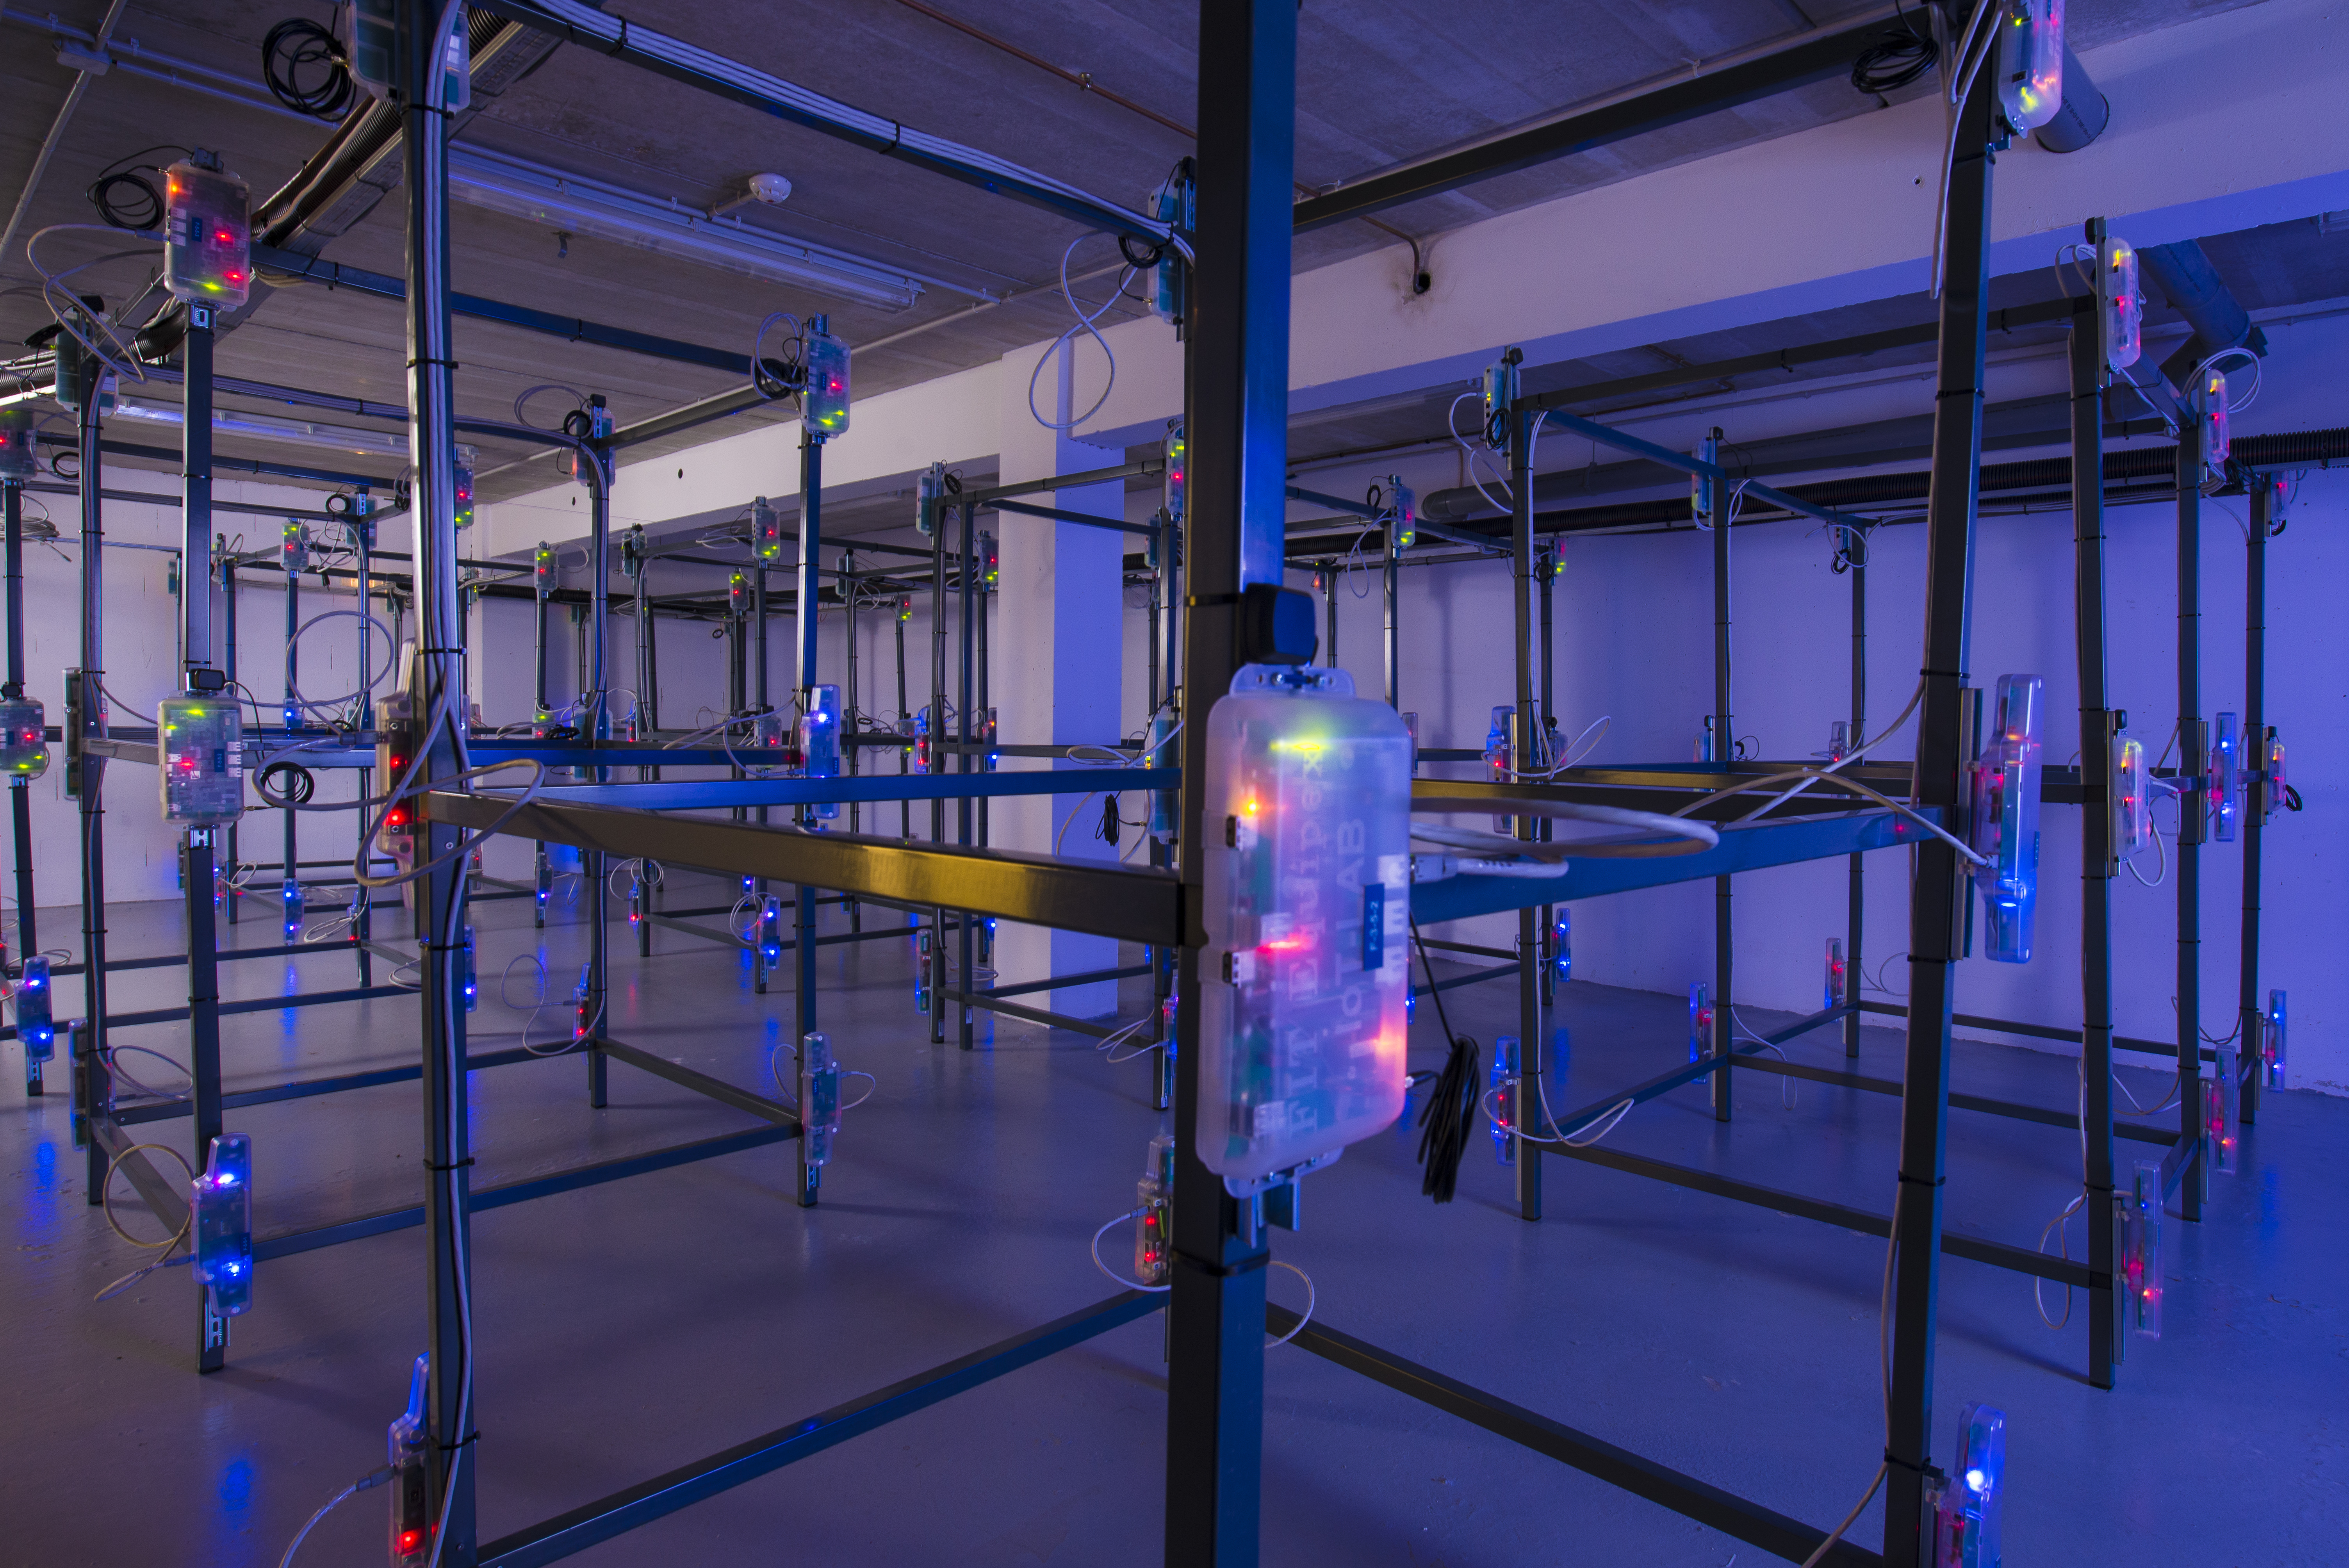
\includegraphics[width=\textwidth]{figures/iotlab.jpg}
  \end{figure}

  \pnote{
    - Testbed où on teste les protocoles sur des plateformes matérielles diverses
  }
  \pnote{
    - Déploiement simplifié permettant un passage à l'échelle plus simple.
  }

\end{frame}

\begin{frame}\frametitle{Domaines d'application}

    \begin{block}{Applications industrielles}
      Mesures, Controle des chaines de productions
    \end{block}
  
    \begin{block}{Villes intelligentes}
      Voirie, Controle de l'eau, Smart parking
    \end{block}
  
    \begin{block}{Gestion de bâtiment}
      Alarmes, chauffage, lumière, surveillance, fermeture des portes
    \end{block}
  
    \begin{block}{Communications Machine to Machine (M2M)}
      Découverte et autoconfiguration de services
    \end{block}
  



  % \begin{itemize}
  %   \item Applications industrielles
  %   \item Villes intelligentes
  %   \item Gestion de bâtiment (Domotique ou professionels)
  %   \item Communications Machine to Machine (M2M)
  % \end{itemize}

  \pnote{
    Insister sur le fait que les applications  sont très diverses et toujours orientées vers un service pour justifier de manière tangible un investissement.
  }
  
\end{frame}

\begin{frame}{Architecture générale}
  \begin{figure}
    \centering
    \includegraphics[scale=.75]{figures/architecture_general_slides.pdf}
  \end{figure}

  \pnote{
    - Quand ces systèmes ne sont pas autonomes il faut une interconnexion on appelle cela une passerelle.
  }

\end{frame}

\begin{frame}{Challenges}

  \begin{block}{Contraintes matérielles}
    \begin{itemize}
      \item Grande hétérogéneité
      \item Faibles ressources matérielles
      \item Batterie ou source d'alimentation limitée
    \end{itemize}
  \end{block}  

  \begin{alertblock}{Solutions}
    \begin{itemize}
      \item Standards de communications
      \item Système d'exploitation adaptés
      \item Cycle de sommeil
    \end{itemize}
  \end{alertblock}

  \pnote{
    - L'hétérogéneité provient de la profusion des acteurs et du faible cout d'entrée dans les marchés
  }
  \pnote{
    - Dire que les progrès technologiques visent à rendre les composants moins chers au lieu de performants
  }    
  \pnote{
    - En raison de la variété des standards il faut des systèmes qui s'autoconfigure autant que possible pour faciliter l'accès.
  }    
  \pnote{
    - La gestion du cycle de vie (authentification, mises à jour, facturation) doivent etre automatisées autant que possibles autrement elles seront jamais     faites cependant la bande passante peut etre critique.
  }

\end{frame}

\begin{frame}{Contraintes liées aux réseau}

  \begin{block}{Contraintes liées aux réseau}
    \begin{itemize}
      \item Faible bande passante
      \item Noeud en sommeil (Connexions intermittantes)
      \item Canal bruité
      \item Passage à l'échelle
    \end{itemize}
  \end{block}

  \begin{alertblock}{Solutions}
    \begin{itemize}
      \item Protocoles réseau adaptés
      \item Couche MAC adaptée
    \end{itemize}
  \end{alertblock}

  \pnote{
    - Faible puissance d'emission
  }
  \pnote{
    - Liens assez mauvais et bruité
  }
  \pnote{
    - Mentionner les problèmes de multi-path fading
  }
\end{frame}

\begin{frame}{Problématiques}
  \begin{block}{Connaitre l'état des noeuds}
    \begin{itemize}
      \item Diagnostiquer ou anticiper des pannes
      \item Mesurer les grandeurs caractéristiques
      \item Provisionner le réseau contraint
    \end{itemize}
  \end{block}

  \begin{block}{Comment optimiser l'utilisation des ressources de ces réseaux contraints ?}
    \begin{itemize}
      \item Limiter la charge sur les noeuds contraints
      \item Conserver un niveau de service suffisant
    \end{itemize}
  \end{block}

\end{frame}

\begin{frame}{Axes des contributions}
  \begin{block}{Passerelle}
    \begin{itemize}
      \item Interface entre les réseaux contraints et classiques
      \item Services pour le réseau de capteurs
    \end{itemize}
  \end{block}

  \begin{alertblock}{Axes de contributions}
    \begin{itemize}
      \item Ajout de fonctionnalités transparentes pour le réseau de capteurs
    \end{itemize}
  \end{alertblock}

  \pnote{
    - Position clé à mi chemin entre le monde contraint et le monde non contraint.
    Plus facile d'y accéder qu'au noeuds contraints.
  }
  
  \pnote{
    Plus ressources car doit par exemple fournir une connectivité permanente par réseaux cellulaires, Ethernet. 
    Services supplémentaires: Pare-feux, sauvegarde des données collectées, mises à jour firmware, synchronisation d'horloge, 
    routeur de sortie, etc.
  }
  \pnote{
    - Comment ajouter des fonctionnalités utiles et transparentes pour les noeuds ?
  }

\end{frame}